\chapter{Implementácia} \label{chapter:implementation}
Firmvér senzorovej jednotky je implementovaný v programovacom jazyku C so
SDK Espressif IoT Development Framework (ESP-IDF). Súbežný beh úloh spravuje operačný systém reálneho času FreeRTOS.
Optimalizované rutiny spracovania signálu poskytuje Espressif DSP Library. Knižnica MPack má na starosti
kódovanie a dekódovanie formátu Message Pack. CMake riadi zostavovanie
modulov zdrojového kódu. Eclipse Mosquitto pôsobí ako MQTT broker správ.

V jazyku Python sú napísané Jupyter notebooky na analýzu zozbieraných datasetov a otestovanie fáz navrhnutej dátovej pipeline,
so závislosťami numpy, scipy, pandas a matplotlib. Rozhranie príkazového riadku na nahrávanie konfigurácie a náhľad odoberaných
správ sa spolieha na balíčky Paho MQTT, cmd a msgpack.

\section{Senzorová sieť}
Súčiastky FireBeetle ESP32, OpenLog, STEVAL-MKI159V1 a BTS117 sú naspájkované na univerzálny plošný spoj rozmerov 5 x 7 cm
(obr. \ref{board}). Doska je vsadená do plastovej krabičky s hrúbkou stien 3 mm vo výške 2 cm nad povrchom.
Akcelerometer je namontovaný tesne pod modulom MCU. Externý 5 V zdroj sa pripája cez Micro USB konektor, alebo 3,7 V lítiovú batériu 
zapojíme cez JST PH 2 pin.
\begin{figure}[h!]
\centering
\begin{subfigure}{0.6\textwidth}
    \centering
    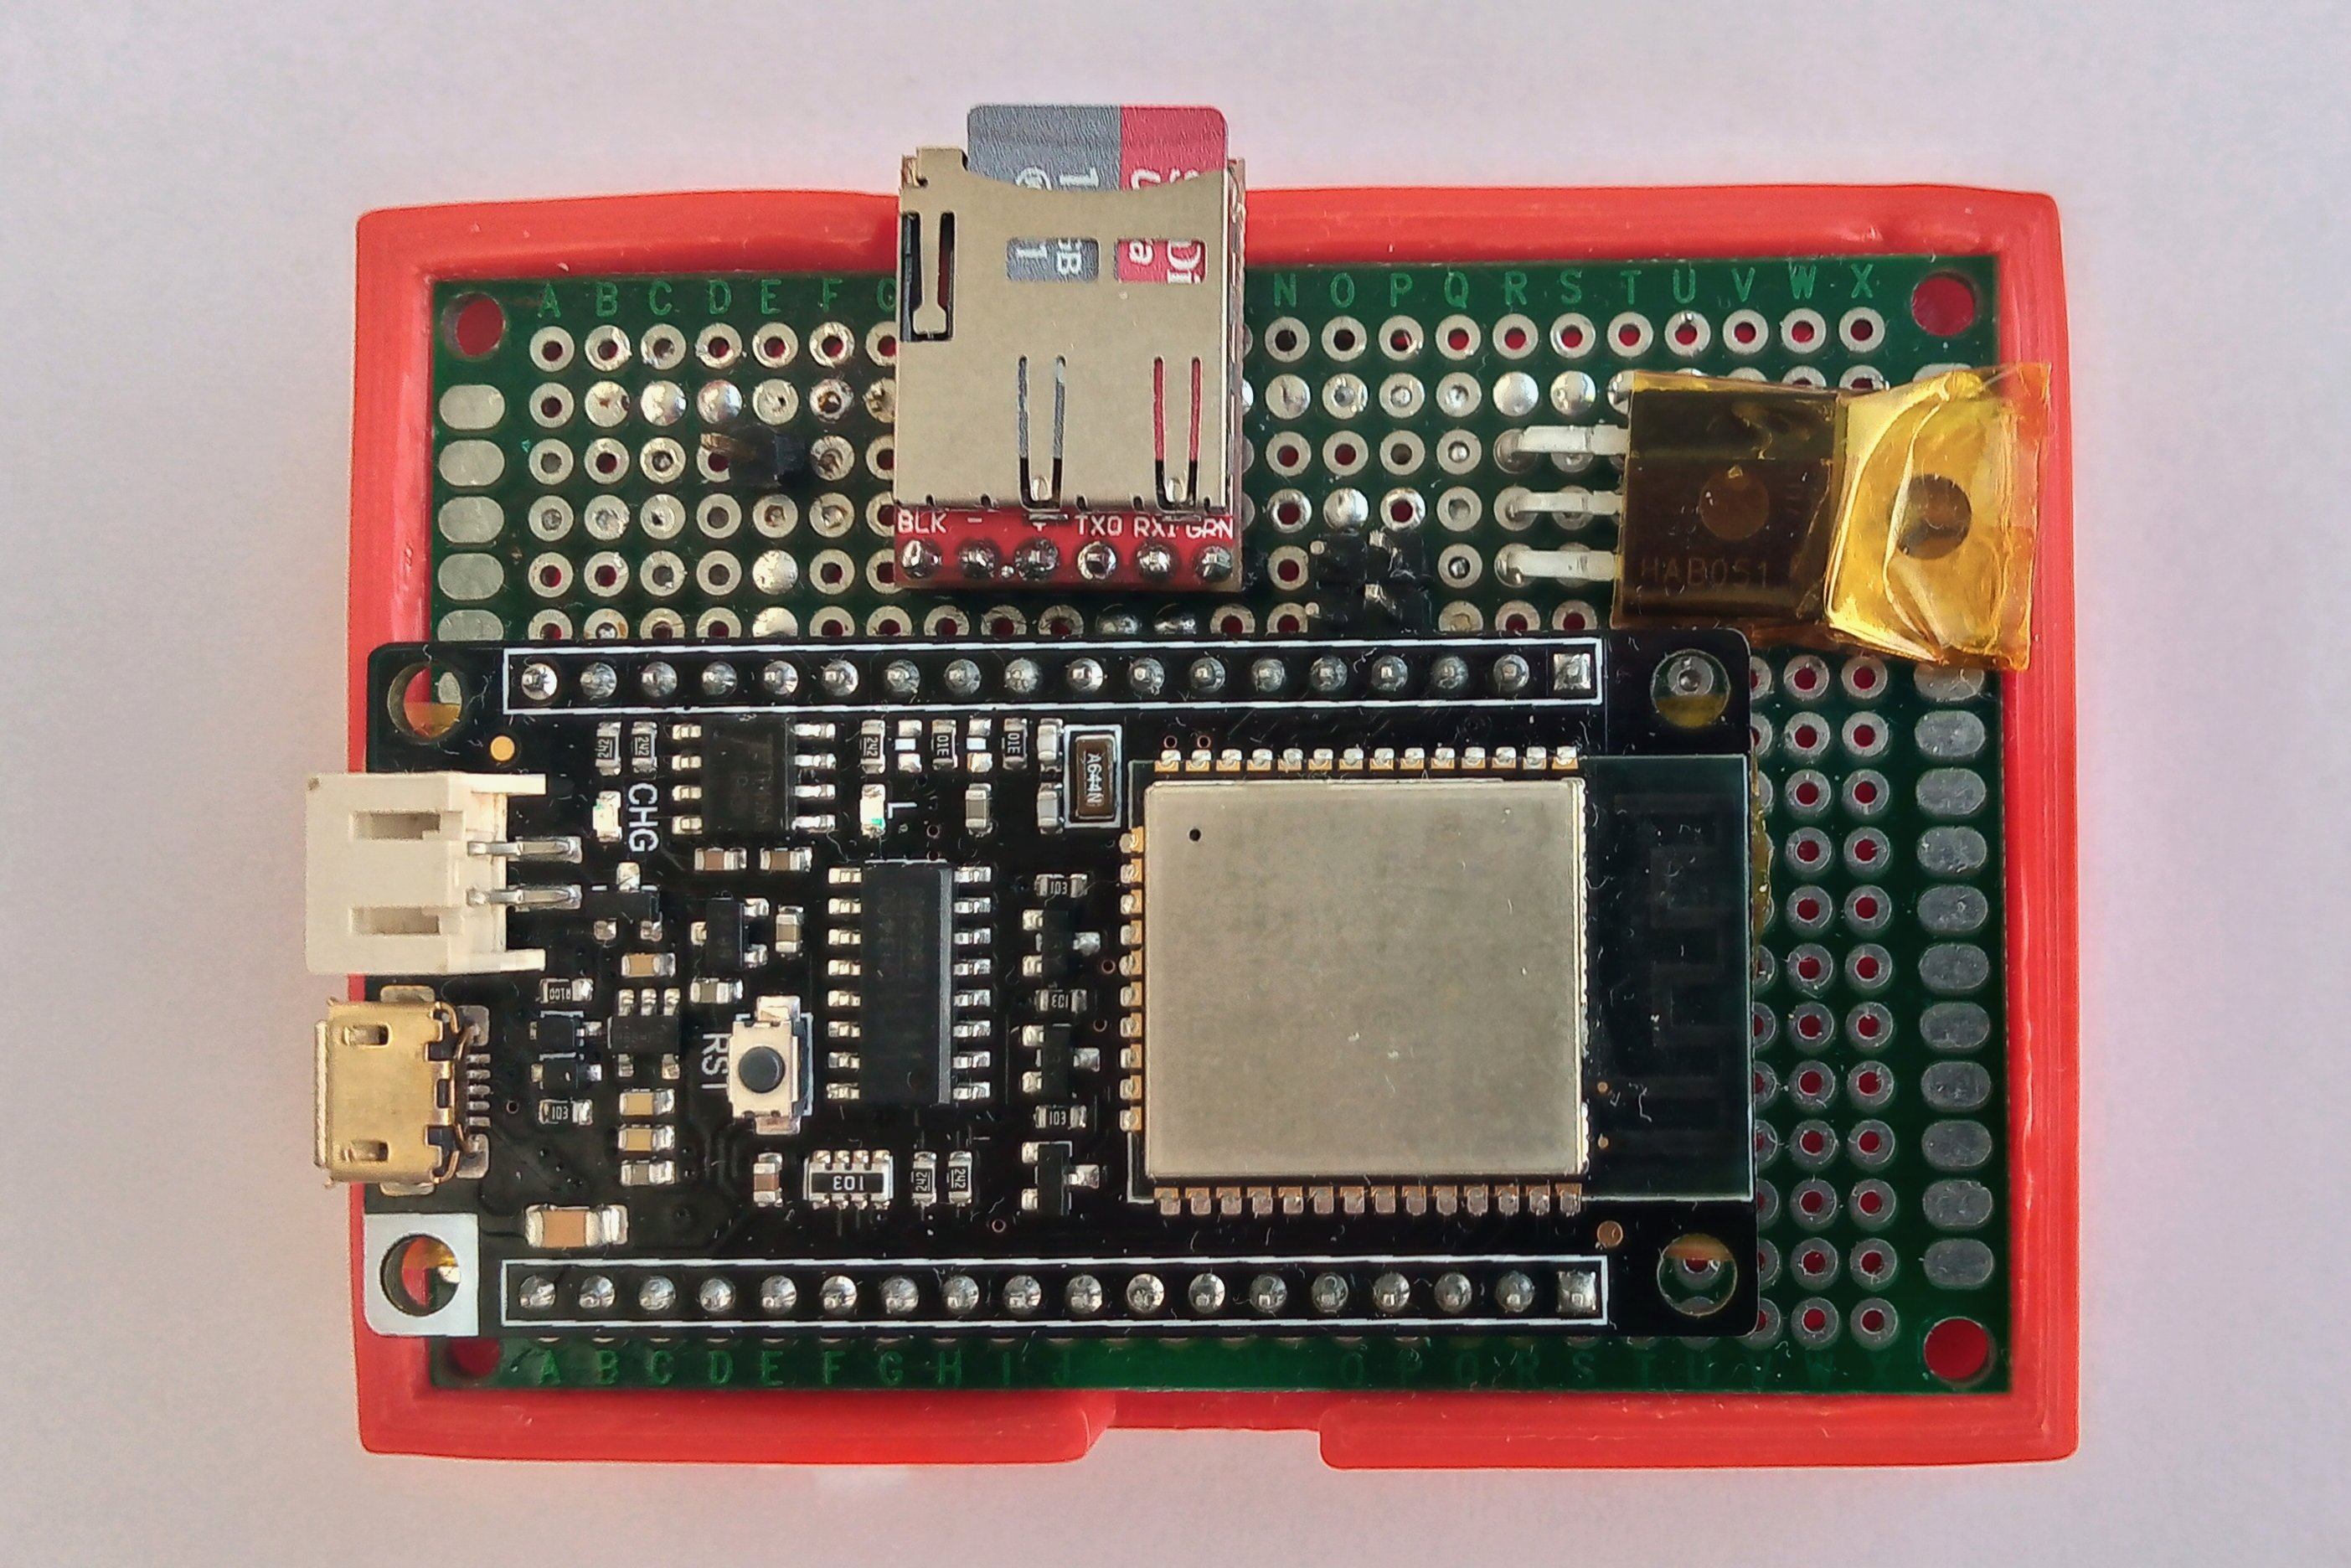
\includegraphics[width=\textwidth]{figures/design/esp32.jpg}
\end{subfigure}
\begin{subfigure}{0.2\textwidth}
    \centering
    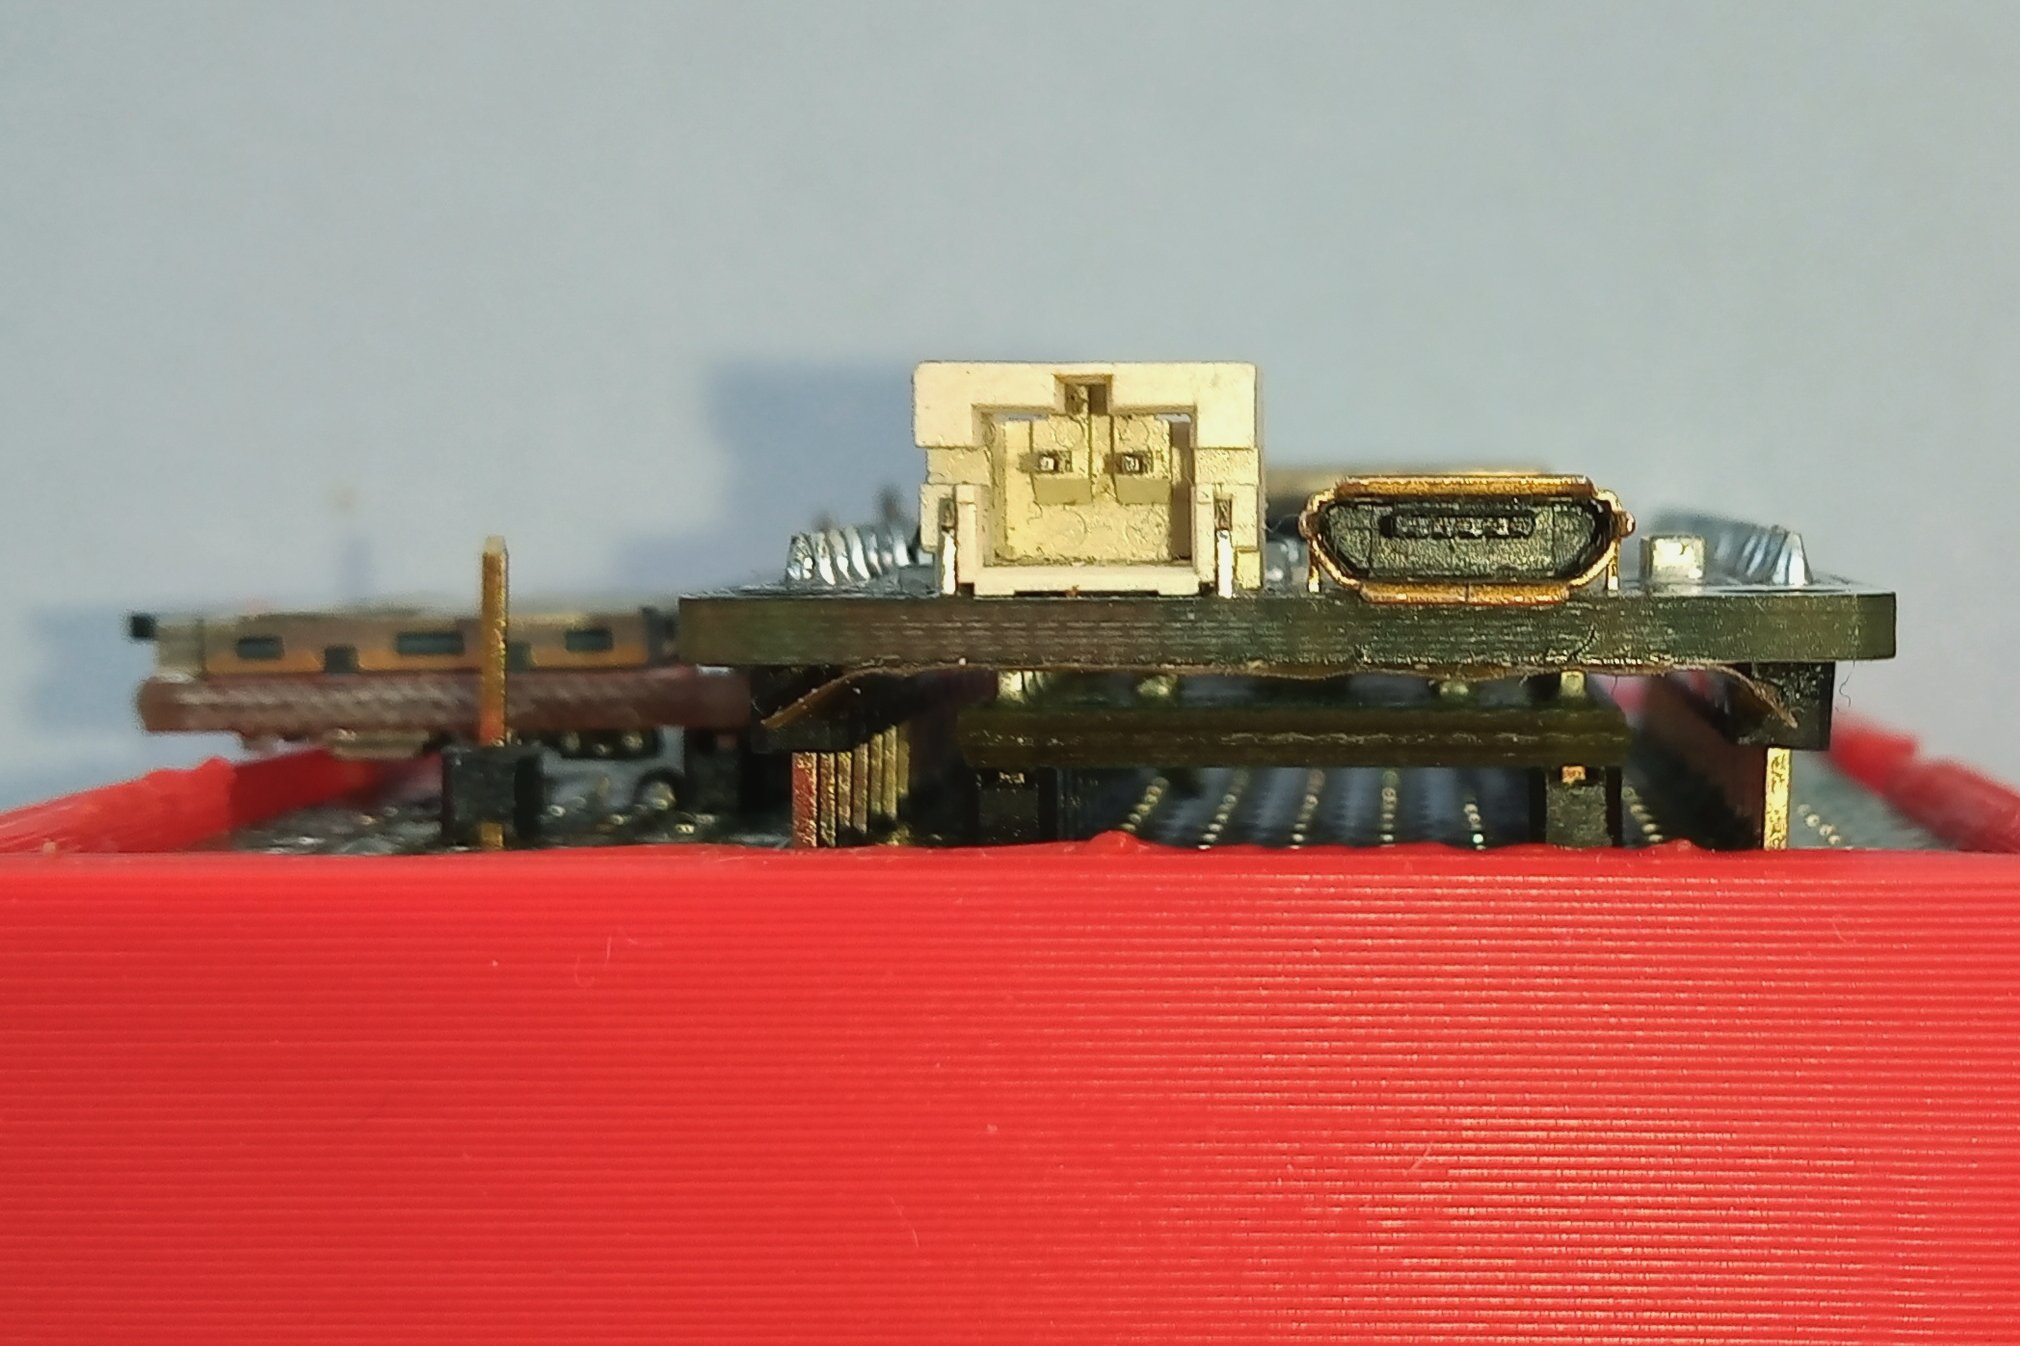
\includegraphics[width=0.9\textwidth]{figures/design/esp32-front.jpg}
\end{subfigure}
\caption{Univerzálny plošný spoj v krabičke osadený modulmi}
\label{board}
\end{figure}

Po zapnutí si firmvér načíta systémové nastavenia cez SDK Storage API z flash. Inicializuje sa
akcelerometer a naraz sa kompletne alokuje dynamická pamäť pre výpočty dátovej pipeline a pre synchronizačné primitíva.
Na zamedzenie fragmentácie nie je odvtedy programom prideľovaná žiadna ďalšia pamäť okrem zásobníkov úloh.

Prebehne pokus o pripojenie s prístupovým bodom WiFi so zabezpečením WPA2 a so serverom MQTT broker, na základe prihlasovacích údajov
a URL adresy v štruktúre \verb|Provisioning|. Proces spustenia OpenLog čaká po zopnutí napájania 10 sekúnd na uvedenie
periférie do prevádzkyschopného stavu.
\begin{lstlisting}[style=implementation]
Provisioning login = {
    .wifi_ssid="AccessPoint",
    .wifi_pass="password",
    .mqtt_url="mqtt://192.168.1.2:1883"
};
\end{lstlisting}

Priame prepísanie predvolenej hodnoty systémového nastavenia v zdrojovom kóde
sa po nahratí firmvéru neprejaví za behu. Predtým sa musí naflashovať obslužný program vyvolaní direktívou
\verb|FACTORY_RESET| pri kompilácii, ktorý premietne tieto nastavenia do partície nevolatilnej pamäte.

Broker MQTT správ Eclipse Mosquitto nasadený v lokálnej sieti, má umožnené cez konfiguračný súbor \verb|mosquitto.conf| počúvať
premávku zo všetkých IP adries na TCP porte 1883, bez nutnosti klientov sa autentifikovať:
\begin{lstlisting}[style=implementation]
listener 1883 0.0.0.0
allow_anonymous true
\end{lstlisting}

Vlastný MQTT klient \verb|config_tool.py| je interpreter príkazov na interaktívnu interakciu so senzorovými jednotkami
pripojenými na broker. Ponúka nadstavbu nad binárnymi správami v Message Pack konverziou z a do ľudsky čitateľnejšej
podoby vo formáte JSON. Povelom \emph{connect} dôjde k nadviazaniu spojenia s brokerom správ, za filtrovania topics podľa
zadaného identifikátora zariadenia. Prefix MQTT tém definuje konštanta firmvéru \verb|DEVICE_MQTT_TOPIC|, ktorý konvenčne začína
s ,,imu/[Device ID]/''.

Režim na nastavenie systémovej konfigurácie IoT koncového uzla sa vyvolá povelom \verb|set| a dopyt aktuálnych pravidiel
príkazom \verb|config|. Po aplikovaní zmien sa čaká sa opätované nabehnutie systému alebo chybovú hlášku.
Zobrazenie jednotkou publikovaných údajov na MQTT tému alebo skupinu tému sa určuje povelom \verb|topic|.

Na SD karte data loggera sa nachádza súbor \verb|config.txt| s uvedenou znakovou rýchlosťou
rovnakou ako pre UART zbernicu mikrokontoléra. Preferované nastavenia sú najvyššia prenosová rýchlosť 115000
v móde 0 zakladajúcom nový log súbor po reštarte:
\begin{lstlisting}[style=implementation]
115200,36,3,0,1,1,0
baud,escape,esc#,mode,verb,echo,ignoreRX
\end{lstlisting}

\section{Komunikácia medzi úlohami}
Nezávislé činnosti aplikácie sú prerozdelené medzi vlákna, ktoré si cez fronty posielajú súradnice zrýchlenia.
FreeRTOS úlohy sú funkcie vykonávajúce opakované sekvenciu príkazov v nekonečnom cykle.

Procedúra obsluhy prerušenia hardvérového časovača nesmie čakať, preto je načítaná rovno z IRAM a upovedomí úlohu vzorkovania
(kód \ref{lst:sampling}). Prevzatím notifikácie synchrónne pošle riadiace slovo senzoru na sekvenčné odčítanie celého vektora
akcelerácie od bázovej adresy registra x-ovej osi. Získaná trojica 16-bitových slov sa podľa aktuálneho rozlíšenia prevedie
do štandardnej fyzikálnej jednotky v type \verb|float|.

\begin{lstlisting}[style=cstyle,caption=Posielanie vzoriek medzi úlohami cez fronty,label={lst:sampling},
 morekeywords={ulTaskNotifyTake,xQueueSend,xQueueReceive,buffer_shift_left,p.stream}]
// Sampling task
if (ulTaskNotifyTake(pdTRUE, portMAX_DELAY)) {
	imu_acceleration(&imu, &axis[0], &axis[1], &axis[2]);
	for (i = 0; i < AXIS_COUNT; i++) {
    	if (conf.sensor.axis[i])
        	xQueueSend(pipeline.queue[i], &axis[i], 0);
    }
}
// Pipeline task
if (xQueueReceive(k->queue[x], &p.stream[idx], portMAX_DELAY)) {
	if (++idx < conf.sensor.n) continue;
    // Process buffer p.stream
    buffer_shift_left(p.stream, conf.sensor.n, leftover);
    idx = conf.sensor.n - leftover;
}
\end{lstlisting}
Vkladanie vzoriek do fronty neblokuje, lebo sa nepočíta s úplným vyčerpaním voľných slotov. Posiela sa do fronty
iba vtedy, ak beží úloha pipeline pre danú dimenziu. Na opačnom konci fronty sa čísla po jednom pripájajú do
cirkulárnej vyrovnávacej pamäte. Pole sa prenechá zvyšku úlohy na spracovanie až po naplnení
dosiahnutím \verb|conf.sensor.n| položiek.

Dokončením analýzy posuvného okna sa presunú ponechané hodnoty z prekryvu časových úsekov na začiatok
poľa: $\mathrm{leftover} = n \cdot (1 - \mathrm{overlap})$. Ďalej sa pokračuje prepisovaním už nepotrebných čísel od pozície \verb|idx|.

\begin{lstlisting}[style=cstyle,caption=Synchronizácia úloh na výpočet korelácie osí,label={lst:correlation},
morekeywords={xEventGroupSync}]
xEventGroupSync(barrier, (1 << axis), task_mask, portMAX_DELAY);
	float avg = mean(buffer, n);
	std[axis] = sqrt(variance(buffer, n, avg));
	for (uint16_t i = 0; i < n; i++)
		diff[axis][i] = (buffer[i] - avg);
xEventGroupSync(barrier, (1 << axis), task_mask, portMAX_DELAY);

if (axis[0] && axis[1])
   stats->corr_xy = correlation(diff[0],diff[1],n,std[0],std[1]);
\end{lstlisting}

Okrem synchronizácie úloh posielaním správ cez fronty sa zužitkúvajú bariéry. Event Groups riadia toky
synchronizovaných úloh v bodoch stretu čakaním na nastavenie bitov podľa očakávanej bitovej masky. Počas
autorizácie voči prístupovému bodu WiFi čaká podprogram hlavného vlákna na príznak pridelenia IP adresy
od obsluhy udalosti nadviazania spojenia.

Koordinácia vlákien je nevyhnutná tiež pri výpočte korelácie, pretože každá os je spracovaná nezávisle. Proces
prezentuje zjednodušený kód \ref{lst:correlation}.V sekcii medzi bariérami si úlohy predpočítajú smerodajnú odchýlku a zoznam rozdielov
od aritmetického priemeru. Konštanta \verb|task_mask| značí bitovými vlajkami, ktoré osi sú aktivované.
Na základe $\mathrm{axis} \in \{0,1,2\}$ signalizuje konkrétne vlákno, že prišlo ku bariére. Mimo kritickej oblasti
si jednotlivé vlákna, disponujúce medzivýsledkami za každú zložku vektora, dorátajú momentálne povolené
kombinácie dvojíc súradníc individuálne.

\section{Udalosti vo frekvenčnom spektre}
ESP DSP knižnica optimalizuje pre naše účely transformáciu do frekvenčnej domény, algoritmami FFT s radixom 2 alebo DCT-II,
a vyhladenie signálu konvolúciou. Avšak dostupná implementácia kosínusovej transformácie nie je adekvátna.
Vyžaduje štvornásobnú veľkosť tabuľky koeficientov ku veľkosti transformácie a vnútorne volá generický
algoritmus FFT. Prišlo k úprave zdrojového kódu knižnice, aby sa aspoň použila platforme prispôsobená verzia.

Pred oboma typmi transformácii sa vynásobia vzorky v posuvnom okne s pripravenými váhami oknovej funkcie (kód \ref{fft}).
Líši sa spôsob napĺňania vstupného poľa, kde u FFT tvoria reálne čísla na párnom a nepárnom mieste za sebou
spoločné komplexné číslo. DCT ponecháva následnosť reálnych vstupov, zato prázdna druhá polovica poľa zostáva
na pracovné účely funkcie.

Poradie vedierok výsledného spektra FFT sa musí explicitne bitovo invertovať a previesť späť na striedanie
reálnych a imaginárnych zložiek. Na záver sú zistené magnitúdy komplexných čísel.
Prepočet na decibely berie za referenčnú úroveň frekvenciu s najväčšou intenzitou.

\begin{lstlisting}[style=cstyle,label={fft},caption=Fourierová a kosínusová transformácia s ESP DSP knižnicou]
case DFT:
	for (uint16_t i = 0; i < n; i++) {
		spectrum[2*i+0] = buffer[i] * window[i];
		spectrum[2*i+1] = 0;
	}
	dsps_fft2r_fc32_ae32(spectrum, n);
	dsps_bit_rev2r_fc32(spectrum, n);
	dsps_cplx2reC_fc32(spectrum, n);
case DCT:
	for (uint16_t i = 0; i < n; i++)
    	spectrum[i] = buffer[i] * window[i];
    dsps_dct_f32(spectrum, n);
\end{lstlisting}

Stav detektora udalostí pozostáva z poľa štruktúr \ref{event:struct}, ktoré odvádzajú časové značky
počiatku, trvania a naposledy videnej špičky od počítadla prebehnutých posuvných okien. Upozornenie na
zmeny vo frekvencii sa pri prechode prúdovým algoritmom poznačí do vymenovaného typu
aktuálnej akcie \verb|SpectrumEventAction|. Nadobúda konštanty z množiny ,,nič'', ,,štart'' alebo ,,koniec'' a
obnovujú sa na začiatku každého ďalšieho kola, na stav neprítomnosti akejkoľvek zmeny. Udalosti na odoslanie
sú síce pri serializácii správy lineárne prehľadávané, ale vytráca sa potreba udržiavať zásobník emitovaných udalostí.

\begin{lstlisting}[style=cstyle,label={event:struct},
caption={Štruktúra udalosti frekvenčného vedierka},morekeywords={SpectrumEvent}]
typedef struct {
    SpectrumEventAction action;
    uint32_t start;
    uint32_t duration;
    int32_t last_seen;
    float amplitude;
} SpectrumEvent;
\end{lstlisting}

\section{Systémová konfigurácia}
Správanie blokov dátovej pipeline určuje globálna inštancia zloženej štruktúry \emph{Configuration} \ref{config:struct}.
Vnorené členské premenné definujú vlastnosti jednotlivých funkčných blokov. Po zapnutí je posledná
konfigurácia zobraná ako blob z nevolatilnej pamäte pod kľúčom ,,config''. Chýbajúca podpora iných ako celočíselných
typov znamená, že po akejkoľvek úprave musí byť štruktúra znovu nahratá do flash pamäte ako celok.

\begin{lstlisting}[style=cstyle,label={config:struct},caption=Štruktúra systémovej konfigurácie,
morekeywords={Configuration}]
typedef struct {
    SamplingConfig sensor;
    SmoothingConfig tsmooth;
    StatisticsConfig stats;
    FFTTransformConfig transform;
    SmoothingConfig fsmooth;
    EventDetectionConfig peak;
    SaveFormatConfig logger;
} Configuration;
\end{lstlisting}

Názvy, typy a prípustné hodnoty atribútov vo formáte Message Pack sú vyjadrené imperatívne priamo vo funkciách
na konštruovanie a rozklad reťazca dátového obsahu paketu. Parsovanie prebieha v jednom prechode s MPack Expect API
umožnením flexibilného poradia kľúčov, ktoré umožňuje priradiť modifikované pravidlo do kópie štruktúry bez dodatočného
syntaktického stromu.
